%% \documentclass[handout,t]{beamer} % HANDOUT
%% \documentclass[handout,notes=show,t]{beamer} % NOTES
\documentclass[t]{beamer} % SLIDES
\usepackage{etex}

\usetheme{DSM}
\usepackage{beamer-tools-dsm}

%%
%% some useful macros: mathematical notation etc.
%%

%% abbreviations for logic symbols
\renewcommand{\implies}{\Rightarrow}
\newcommand{\equivalent}{\Leftrightarrow}

%% abbreviations for common number spaces
\newcommand{\setN}[1][]{\mathbb{N}_{#1}} % allows \setN and \setN[0]
\newcommand{\setZ}{\mathbb{Z}}
\newcommand{\setQ}{\mathbb{Q}}
\newcommand{\setR}{\mathbb{R}}

%% sets and (sub-)sets defined by condition
\newcommand{\set}[1]{\{#1\}}
\newcommand{\setdef}[2]{\set{#1\,|\,#2}}
\newcommand{\bigset}[1]{\bigl\{#1\bigr\}}
\newcommand{\bigsetdef}[2]{\bigset{#1\bigm|#2}}
\newcommand{\setscale}[1]{\left\{#1\right\}}
\newcommand{\setdefscale}[2]{\setscale{#1\left|\,#2\right.}}

%% absolute value and norm
\newcommand{\abs}[1]{\lvert #1\rvert}
\newcommand{\bigabs}[1]{\bigl\lvert #1\bigr\rvert}
\newcommand{\absscale}[1]{\left\lvert #1\right\rvert}
\newcommand{\norm}[2][]{\lVert #2\rVert_{#1}}
\newcommand{\bignorm}[2][]{\bigl\lVert #2\bigr\rVert_{#1}}
\newcommand{\normscale}[2][]{\left\lVert #2\right\rVert_{#1}}

%% complement set (with optional index)
\newcommand{\compl}[1][]{\mathcal{C}^{#1}}

%% power set: \powerset{\Sigma^*}
\newcommand{\powerset}[1]{\mathcal{P}(#1)}

%% uparrow: a \ua b = direct dominance in ordered tree
\newcommand{\ua}{\uparrow}

%% left-right arrow: this $\lra$ that
\newcommand{\lra}{\leftrightarrow}

%% expanded engineering notation: 4.2\x\e+5
\newcommand{\e}[2]{10^{\ifthenelse{\equal{#1}{+}}{}{#1}#2}}
\newcommand{\x}{\cdot}

%% arg max & min: \argmax_{x\in C}, \argmin_{x\in C}
\newcommand{\argmax}{\mathop{\text{arg~max}}}
\newcommand{\argmin}{\mathop{\text{arg~min}}}

%% infinitesimal elements: \dx, \dy = \dX{y}, \dz
\newcommand{\dX}[1]{\,\mathit{d{#1}}}
\newcommand{\dx}{\dX{x}}
\newcommand{\dy}{\dX{y}}
\newcommand{\dz}{\dX{z}}

%%% Local Variables: 
%%% mode: latex
%%% TeX-master: ""
%%% End: 
  % basic mathematical notation
%%
%% some macros for typesetting text
%%

%% \OPEN ... \CLOSE; \OPEN[np] ... \CLOSE[np]
%% bold large brackets for labelled bracketing notation
\newcommand<>{\OPEN}[1][]{\only#2{$\boldsymbol{\bigl[}\text{}_{\text{\raisebox{-2pt}{\textsc{#1}}}}$}}
\newcommand<>{\CLOSE}[1][]{\only#2{$\text{}_{\text{\raisebox{-2pt}{\textsc{#1}}}}\boldsymbol{\bigr]}$}}

%% \textgap ("_" representing missing letter)
\newcommand{\textgap}{\mbox{\hspace{.4pt}\texttt{\bfseries\secondary{\textunderscore}}\hspace{.4pt}}}

%% \textstar, \textast (math \star and \ast symbols in text mode, with some extra spacing)
\newcommand{\textstar}{$\mspace{.8mu}\star\mspace{.8mu}$}
\newcommand{\textast}{$\ast$}

%% $\p{\ctext{abc}}$ (cited text in mathematical equations, e.g. n-gram probabilities)
\newcommand{\ctext}[1]{\text{\textcite{#1}}}

%% $\p{\btext{abc}}$ (normal black text even in coloured math environment)
\newcommand{\btext}[1]{\text{\foreground{#1}}} 

%% text subscripts and superscripts (can be used in math and text mode)
\newcommand{\tsup}[1]{\ensuremath{^{\text{#1}}}}
\newcommand{\tsub}[1]{\ensuremath{_{\text{#1}}}}

%%% Local Variables: 
%%% mode: latex
%%% TeX-master: ""
%%% End: 
  % some useful macros for plain text
%%
%% some useful macros: statistical notation
%%

%% \p{X=k};  \pC{X=k}{Y=l};  \bigp{X_i = k};   \pscale{\frac{Z}{S^2}};
%% probability P(X=k) and conditional probability P(X=k|Y=l), also with larger or scaled parentheses
%% \p[\theta]{X=k};  \pC[\text{interpolated}]{X=k}{Y=l};  ...
%% with optional subscripts (for model probability, null probability, etc.)
\newcommand{\p}[2][]{\mathop{\mathrm{Pr}_{#1}}(#2)}
\newcommand{\pscale}[2][]{\mathop{\mathrm{Pr}_{#1}}\!\left(#2\right)}
\newcommand{\bigp}[2][]{\mathop{\mathrm{Pr}_{#1}}\bigl(#2\bigr)}
\newcommand{\pC}[3][]{\p[#1]{#2\,|\,#3}} 
\newcommand{\pCscale}[3][]{\pscale[#1]{#2\left|\,#3\right.\!}} 
\newcommand{\bigpC}[3][]{\bigp[#1]{#2\!\bigm|\!#3}} 

%% \Exp{X};  \Var{X};  \Exp[0]{X};  \Var[0]{X};  
%% \bigExp{X}; \bigVar{X}; \Expscale{X};  \Varscale{X};
%% expectation E[X] and variance V[X], expectation and variance under null hypothesis, 
%% and variants with largeer or scaled brackets
\newcommand{\Exp}[2][]{\mathrm{E}_{#1}[#2]}
\newcommand{\Var}[2][]{\mathop{\mathrm{Var}}_{#1}[#2]}
\newcommand{\bigExp}[2][]{\mathrm{E}_{#1}\!\bigl[#2\bigr]}
\newcommand{\bigVar}[2][]{\mathop{\mathrm{Var}}_{#1}\bigl[#2\bigr]}
\newcommand{\Expscale}[2][]{\mathrm{E}_{#1}\left[#2\right]}
\newcommand{\Varscale}[2][]{\mathop{\mathrm{Var}}_{#1}\left[#2\right]}

%% \pihat = \hat{\pi}
%% sampling estimate for population probability \pi (may need fine-tuning)
\newcommand{\pihat}{\hat{\pi}}

%% \Entropy{X}, \Entropy{p}, \KL{p}{q}, \MI{X}{Y}
%% \bigEntropy{}, \Entropyscale{}, \bigKL{}{}, \KLscale{}{}, \bigMI{}{}, \MIscale{}{}
%% entropy, KL distance, conditional entropy and mutual information (with scaled variants)
\newcommand{\Entropy}[1]{H[{#1}]}
\newcommand{\bigEntropy}[1]{H\bigl[{#1}\bigr]}
\newcommand{\Entropyscale}[1]{H\left[{#1}\right]}
\newcommand{\KL}[2]{D({#1}\|{#2})}
\newcommand{\bigKL}[2]{D\bigl({#1}\bigm\|{#2}\bigr)}
\newcommand{\KLscale}[2]{D\left({#1}\left\|{#2}\right.\right)}
\newcommand{\MI}[2]{I[{#1};{#2}]}
\newcommand{\bigMI}[2]{I\bigl[{#1};{#2}\bigr]}
\newcommand{\MIscale}[2]{I\left[{#1};{#2}\right]}

%% \corr (correlation) and \cov (covariance) as mathop's
\newcommand{\corr}{\mathop{\mathrm{corr}}}
\newcommand{\cov}{\mathop{\mathrm{cov}}
}
%%% Local Variables: 
%%% mode: latex
%%% TeX-master: ""
%%% End: 
  % notation for probability theory and statistics
%%
%% convenience macros for linear algebra (vectors and matrices)
%%

%% \Vector[i]{x} ... vector variable with optional _superscript_ index in parentheses
%% \Vector[']{x} ... special case: ' superscript not enclosed in parentheses
%% \vx, \vy, \vz ... abbreviations for common vector names
\newcommand{\Vector}[2][]{\mathbf{#2}\ifthenelse{\equal{#1}{}}{}{^{(#1)}}}
\newcommand{\vx}[1][]{\Vector[#1]{x}}
\newcommand{\vy}[1][]{\Vector[#1]{y}}
\newcommand{\vz}[1][]{\Vector[#1]{z}}
\newcommand{\vu}[1][]{\Vector[#1]{u}}
\newcommand{\vv}[1][]{\Vector[#1]{v}}
\newcommand{\vw}[1][]{\Vector[#1]{w}}
\newcommand{\va}[1][]{\Vector[#1]{a}} % vectors of coefficients
\newcommand{\vb}[1][]{\Vector[#1]{b}} % for basis
\newcommand{\vc}[1][]{\Vector[#1]{c}} % context vectors
\newcommand{\ve}[1][]{\Vector[#1]{e}} % for standard basis of R^n
\newcommand{\vm}[1][]{\Vector[#1]{m}} % row vectors of term-term matrix
\newcommand{\vn}[1][]{\Vector[#1]{n}} % normal vector
\newcommand{\vmu}[1][]{\Vector[#1]{\boldsymbol{\mu}}} % column vectors of term-term matrix
\newcommand{\vf}[1][]{\Vector[#1]{f}} % row vectors of term-context matrix
\newcommand{\vphi}[1][]{\Vector[#1]{\boldsymbol{\phi}}} % column vectors of term-context matrix
\newcommand{\vxi}[1][]{\Vector[#1]{\boldsymbol{\xi}}} % coordinate vector
\newcommand{\vnull}[1][]{\Vector[#1]{0}} % neutral element

%% \Span{\vb[1],\ldots,\vb[k]} ... span of set of vectors
%% \Rank{...} ... rank of set of vectors or matrix
%% \Det{...}, \det A ... determinant of a set of vectors / a matrix A
%% \Image{f}, \Kernel{f} ... image and kernel of a linear map
\newcommand{\Span}[1]{\mathop{\text{sp}}\left(#1\right)}
\newcommand{\Rank}[1]{\mathop{\text{rank}}\left(#1\right)}
\newcommand{\Det}[1]{\mathop{\text{Det}}\left(#1\right)}
%% \det is already defined in the standard library
\newcommand{\Image}[1]{\mathop{\text{Im}}\left(#1\right)}
\newcommand{\Kernel}[1]{\mathop{\text{Ker}}\left(#1\right)}

%% \dist[2]{\vx}{\vy} ... distance between two vectors (p-metric)
\newcommand{\dist}[3][]{d_{#1}\left(#2, #3\right)}
\newcommand{\bigdist}[3][]{d_{#1}\bigl(#2, #3\bigr)}

%% \sprod{\vu}{\vv} ... scalar product
\newcommand{\sprod}[2]{\left\langle #1, #2 \right\rangle}
\newcommand{\bigsprod}[2]{\bigl\langle #1, #2 \bigr\rangle}


%%% Local Variables: 
%%% mode: latex
%%% TeX-master: ""
%%% End: 
% convenience macros for vectors and matrices

%%%
%%% local configuration adjustments
%%%

%%% You can change pre-defined colours here, override built-in macros from the
%%% style definition and standard library, as well as define macros needed by
%%% all local documents.

%%% e.g. adjust counterpoint (dark green) for data projectors where greens are
%%% far too bright, as well as green component of light colour and pure green
%%% (of course, it's a better solution to adjust the gamma settings of your monitor)
%%
%% \definecolor{counterpoint}{rgb}{.1, .3, 0}
%% \definecolor{light}{rgb}{.45, .3, .55}
%% \definecolor{puregreen}{rgb}{0, .35, 0}

%% ----- extra packages we need to load

\usepackage{tikz}
\usepackage{alltt}              % code examples with nicely formatted comments
\usepackage{hieroglf}           % hieroglyph font for the archeology example
\usepackage{rotating}
\usepackage{multirow}

%% ----- general copyright message (authors may change between versions of the tutorial)
\newcommand{\dsmcopyright}{%
  Copyright \textcopyright\ 2009--2016 Evert, Lenci, Baroni \& Lapesa | 
  Licensed under CC-by-sa version 3.0}


%% ----- automatically show TOC reminder at beginning of each subsection
\AtBeginSubsection[]
{
  \begin{frame}
    \frametitle{Outline}
    \tableofcontents[current,currentsubsection]
  \end{frame}
}

%% ----- some useful macros for the SIGIL course

%% > plot(x,y)      \REM{this produces a scatterplot}
\newcommand{\REM}[2][\small]{\textsf{#1\color{primary}\# #2}}

\newenvironment{Rcode}[1][]{%
\setbeamercolor{block title}{fg=counterpoint,bg=counterpoint!15!white}%
\setbeamercolor{block body}{bg=counterpoint!5!white}\small%
\begin{block}{#1}\begin{alltt}\ungap[1]}{%
\ungap[1]\end{alltt}\end{block}}

%% nice colour for R output: \begin{Rout} .. \end{Rout}
%% -- ugly hack: I'm sure theres a better way to do this
\newenvironment{Rout}[1][\footnotesize]{%
  \begin{footnotesize}#1\color{secondary}\bfseries}{%
  \color{black}\mdseries\end{footnotesize}}

%% symbols for centroid vector and singular value matrix 
%% \newcommand{\vmu}[1][]{\boldsymbol{\mu}\ifthenelse{\equal{#1}{}}{}{^{(#1)}}}
\newcommand{\Msigma}{\boldsymbol{\Sigma}}

%% rotated column labels for table (to fit long text into narrow columns
\newcommand{\rotLabel}[2][60]{\begin{rotate}{#1}#2\end{rotate}}
 % local adjustments to configuration and macros

\begin{document}

%%%%%%%%%%%%%%%%%%%%%%%%%%%%%%%%%%%%%%%%%%%%%%%%%%%%%%%%%%%%%%%%%%%%%%

% %%%%%%%%%%%%%%%%%%%%%%%%%%%%%%%%%%%%%%%%%%%%%%%%%%%%%%%%%%%%%%%%%%%%%%
\section{}

%%%%%%%%%%%%%%%%%%%%%%%%%%%%%%%%%%%%%%%%%%
\subsection{}

\begin{frame}
  \frametitle{}
  % \framesubtitle{}

\end{frame}

\begin{frame}[fragile]
  \frametitle{}
  %% \framesubtitle{}

  % \ungap[1]
  \begin{alltt}
  \end{alltt}
\end{frame}


%%% Local Variables: 
%%% mode: latex
%%% TeX-master: "../workspace"
%%% End: 
 % -- input only slide set you're currently working on
% %%%%%%%%%%%%%%%%%%%%%%%%%%%%%%%%%%%%%%%%%%%%%%%%%%%%%%%%%%%%%%%%%%%%%%
\section{Usage and evaluation of DSM}

%%%%%%%%%%%%%%%%%%%%%%%%%%%%%%%%%%%%%%%%%%
\subsection{What to do with DSM distances}

\begin{frame}
  \frametitle{Nearest neighbours}
  \framesubtitle{DSM based on verb-object relations from BNC, reduced to 100 dim.\ with SVD}
  % \framesubtitle{}

  Neighbours of \h{dog} (cosine angle):
  \begin{itemize}\item[\hand]
    girl (45.5), boy (46.7), horse(47.0), wife (48.8), baby (51.9),
    daughter (53.1), side (54.9), mother (55.6), boat (55.7),
    rest (56.3), night (56.7), cat (56.8), son (57.0), man (58.2), 
    place (58.4), husband (58.5), thing (58.8), friend (59.6), \ldots
  \end{itemize}

  \gap
  Neighbours of \h{school}:
  \begin{itemize}\item[\hand]
    country (49.3), church (52.1), hospital (53.1), house (54.4),
    hotel (55.1), industry (57.0), company (57.0), home (57.7), family
    (58.4), university (59.0), party (59.4), group (59.5), building
    (59.8), market (60.3), bank (60.4), business (60.9), area (61.4),
    department (61.6), club (62.7), town (63.3), library (63.3), 
    room (63.6), service (64.4), police (64.7), \ldots
  \end{itemize}
  \addnote{Neighbours and neighbourhood plots from BNC verb-object DSM, reduced to 100 dimensions by SVD.}%
\end{frame}

\begin{frame}[c]
  \frametitle{Nearest neighbours}
  % \framesubtitle{}

  \begin{center}
    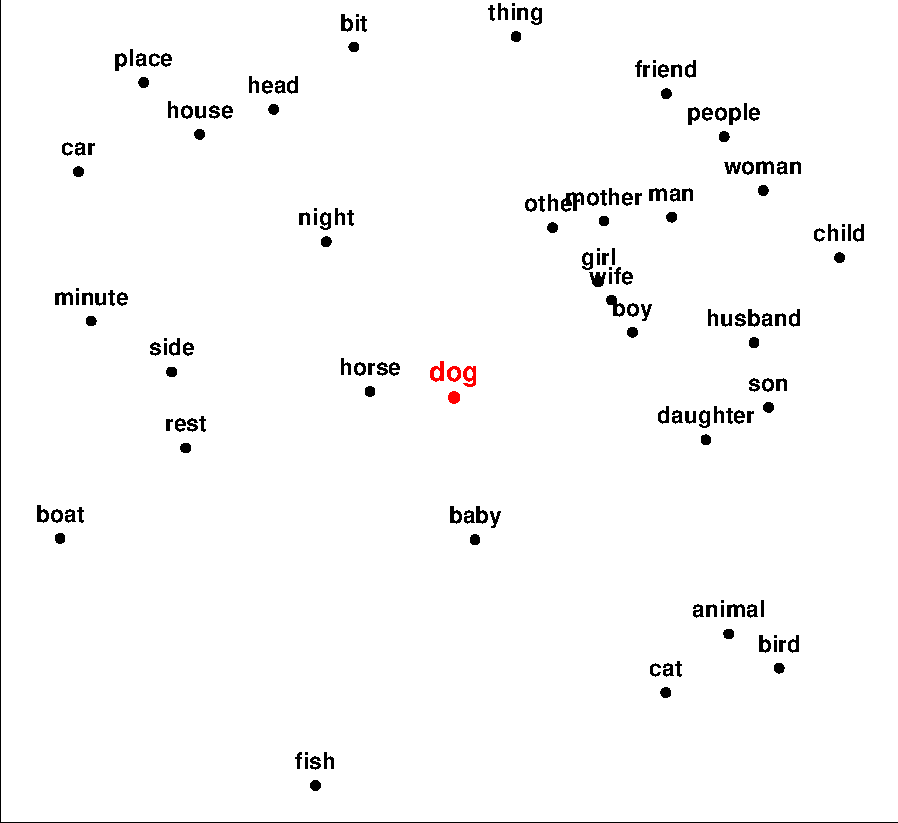
\includegraphics[width=8cm]{img/neighbourhood_dog}
  \end{center}
\end{frame}

\begin{frame}[c]
  \frametitle{Clustering}
  % \framesubtitle{}

  \begin{center}
    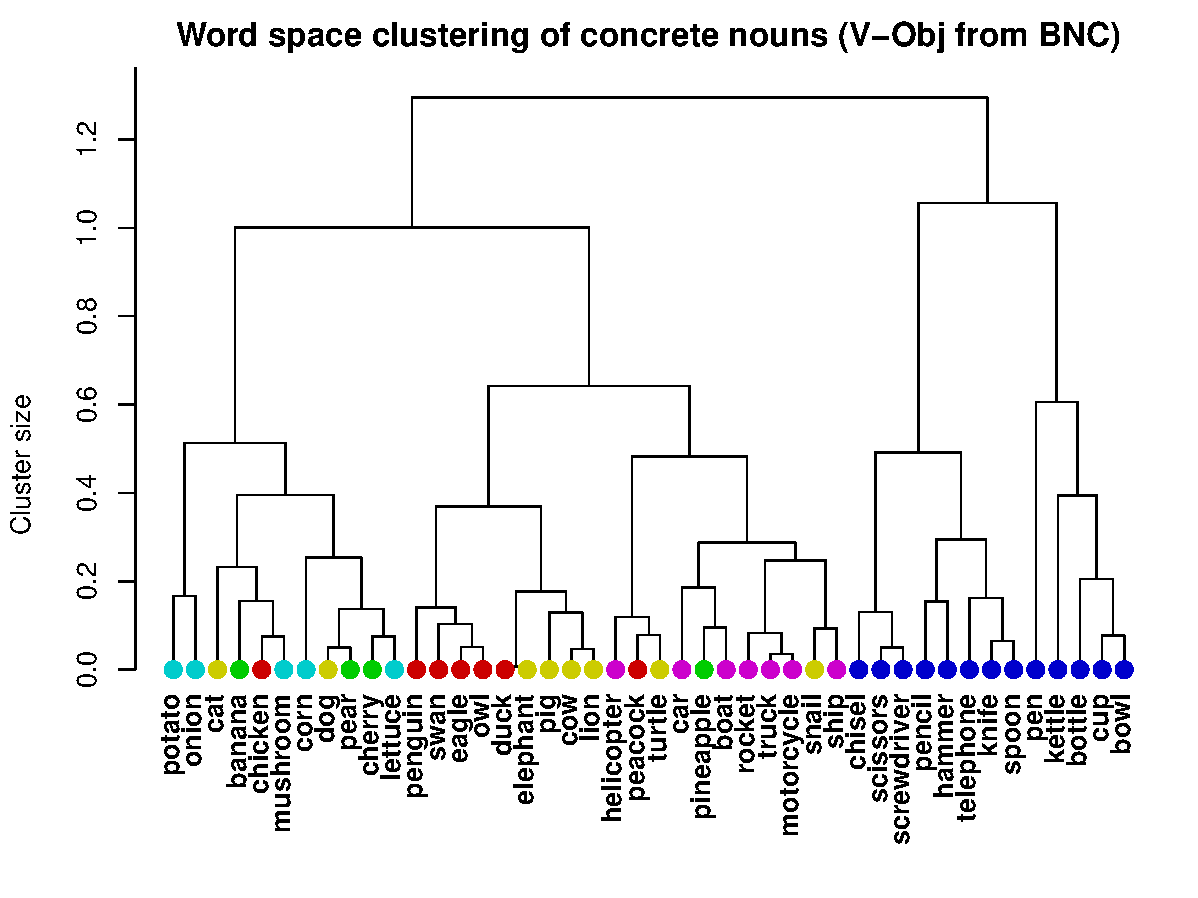
\includegraphics[width=100mm]{img/hieroglyph_clustering}
  \end{center}
\end{frame}

\begin{frame}[c]
  \frametitle{Semantic maps}
  % \framesubtitle{}

  \begin{center}
    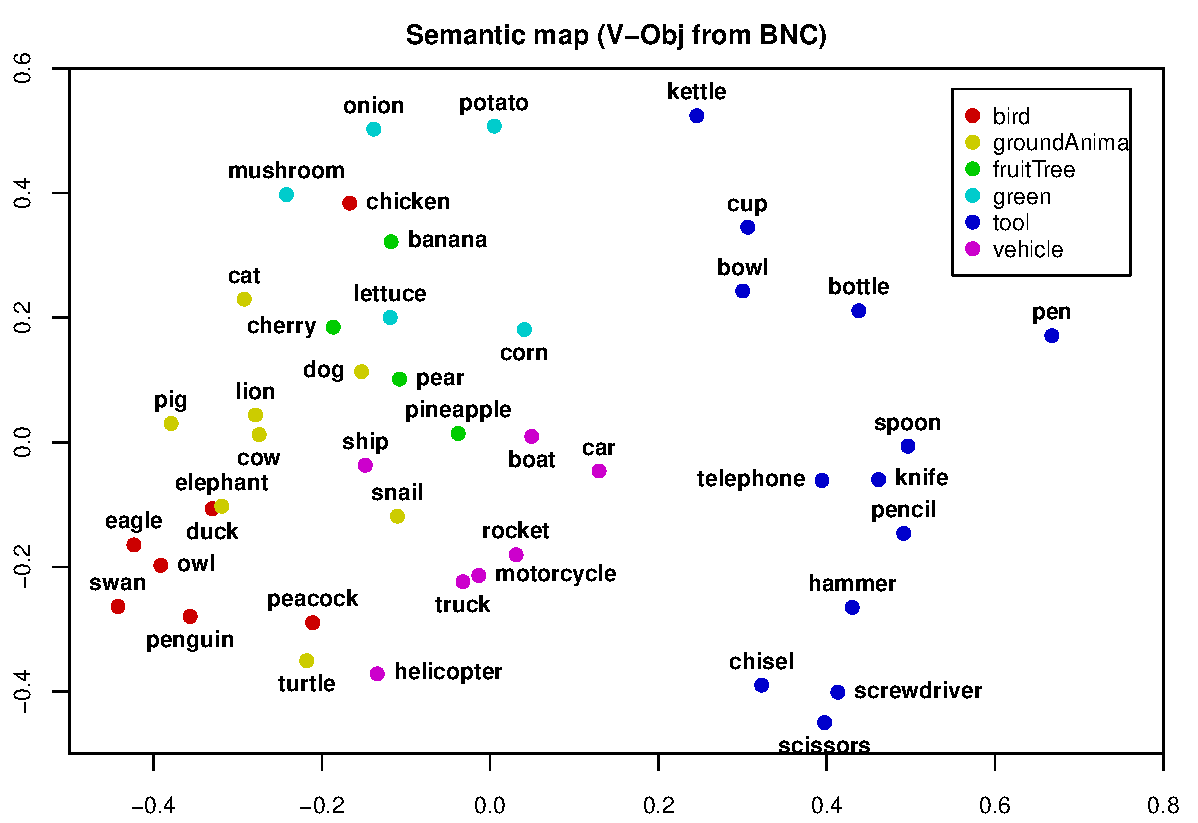
\includegraphics[width=100mm]{img/hieroglyph_semantic_map}
  \end{center}
\end{frame}

\begin{frame}[c]
  \frametitle{Latent dimensions}
  % \framesubtitle{}

  \begin{center}
    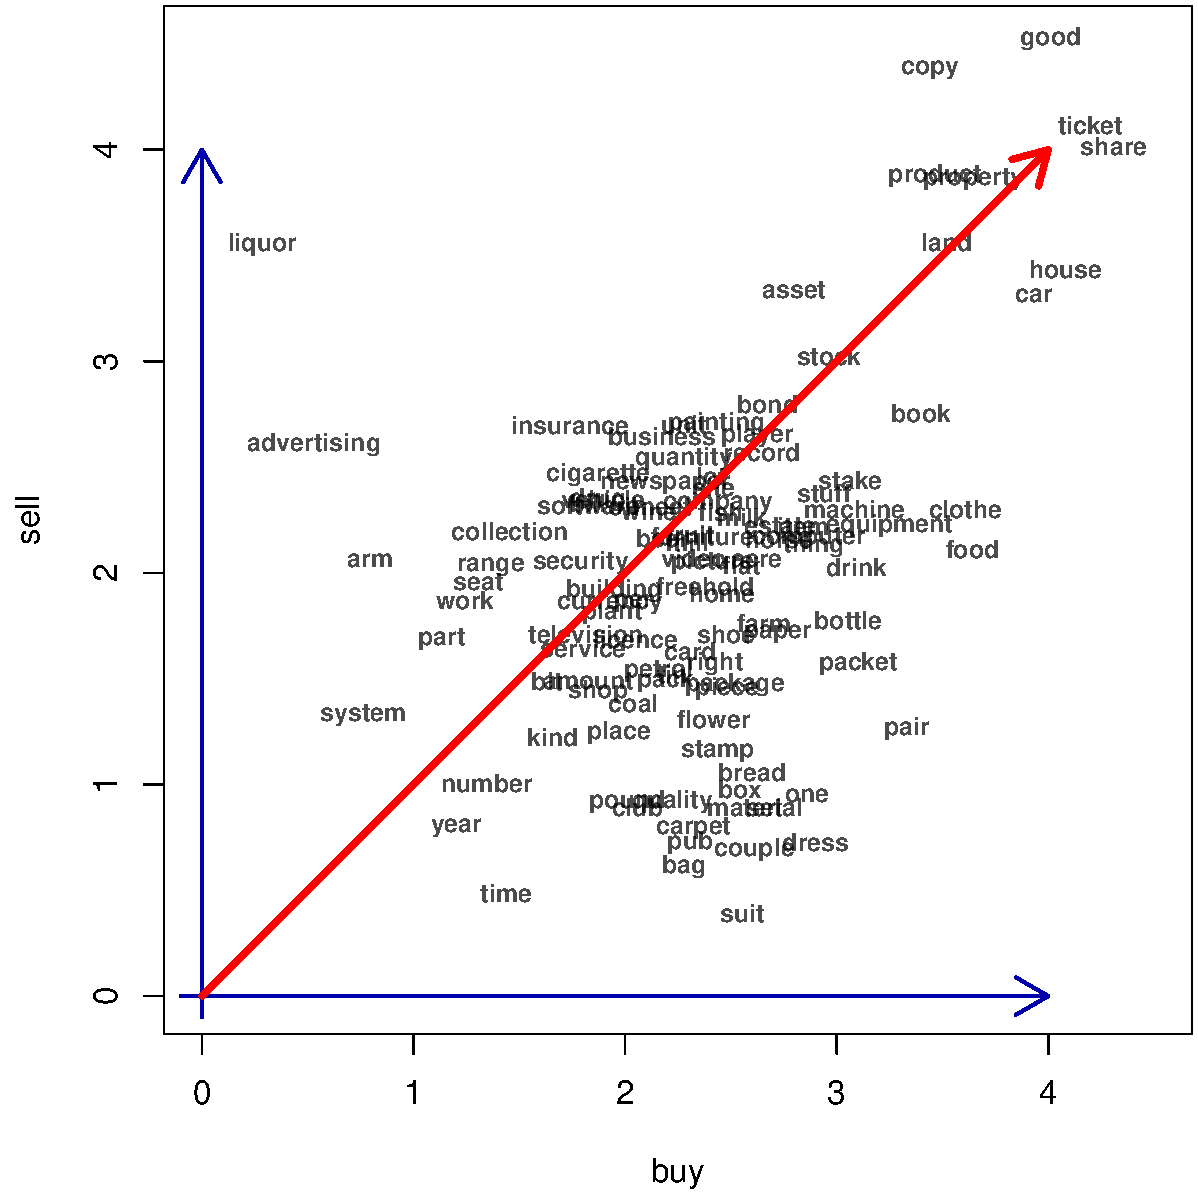
\includegraphics[width=8cm]{img/3_buy_sell_labels_latent}
  \end{center}
\end{frame}

\begin{frame}[c]
  \frametitle{Semantic similarity graph (topological structure)}
  % \framesubtitle{}

  \begin{center}
    \begin{tabular}{@{}cc@{}}
    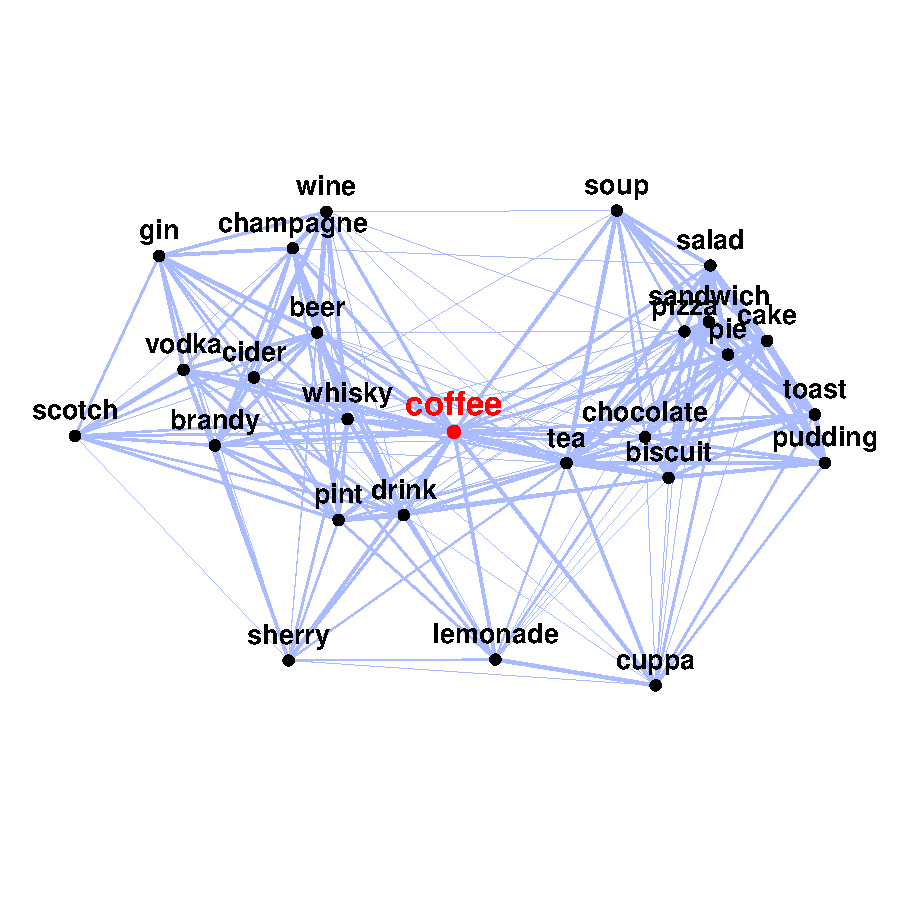
\includegraphics[width=55mm]{img/neighbourhood_coffee} &
    \visible<2->{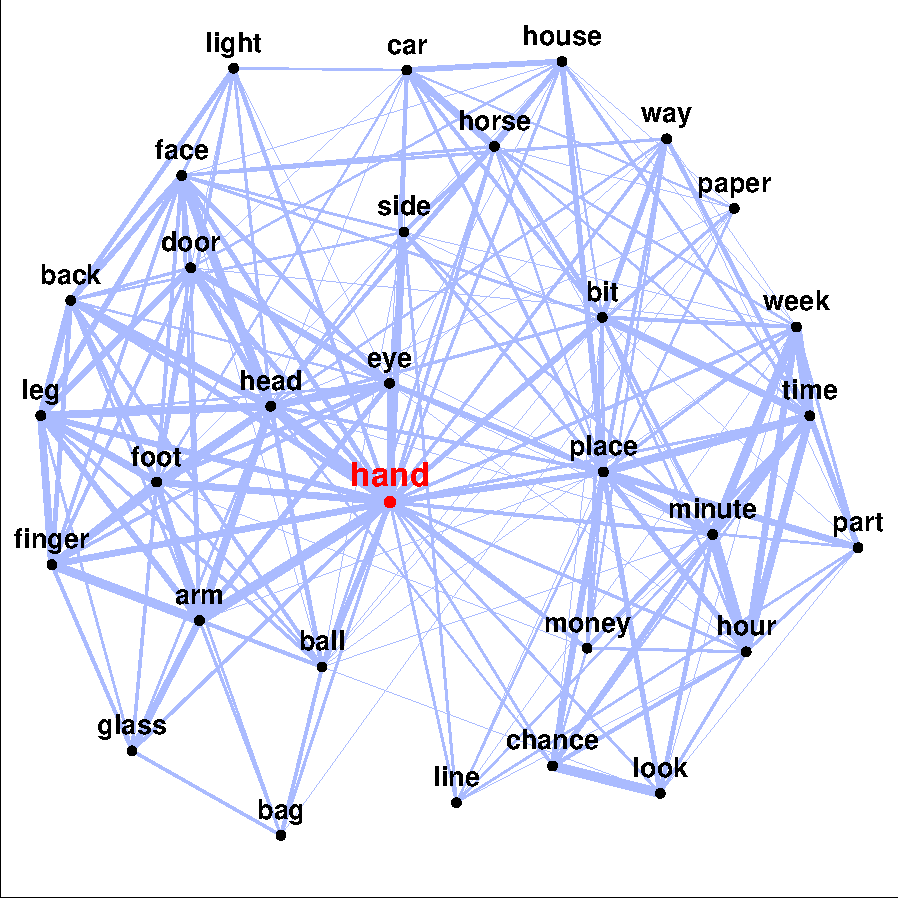
\includegraphics[width=55mm]{img/neighbourhood_hand}}
  \end{tabular}
  \end{center}
\end{frame}



%%%%%%%%%%%%%%%%%%%%%%%%%%%%%%%%%%%%%%%%%%
\subsection{Evaluation: semantic similarity and relatedness}

\begin{frame}
\frametitle{Distributional similarity as semantic similarity}

\begin{itemize}
\item DSMs interpret semantic similarity as a \primary{quantitative notion}
\begin{itemize}
\item if $\va$ is closer to $\vb$ than to $\Vector{c}$ in the distributional
vector space, then $a$ is more semantically similar to $b$ than to $c$
\end{itemize}
\end{itemize}

\begin{center}
  \begin{tabular}{l|l|l}
      \primary{rhino} & \primary{fall} & \primary{rock}\\
      \hline
      woodpecker&    rise&         lava\\
      rhinoceros&    increase&     sand\\
      swan&          fluctuation&  boulder\\
      whale&         drop&         ice\\
      ivory&         decrease&     jazz\\
      plover&        reduction&    slab\\
      elephant&      logarithm&    cliff\\
      bear&          decline&      pop\\
      satin&         cut&          basalt\\
      sweatshirt&    hike&         crevice\\
    \end{tabular}
  \end{center}
\end{frame}


\begin{frame}
\frametitle{Types of semantic relations in DSMs}

\begin{itemize}
\item Neighbors in DSMs have different types of
\primary{semantic relations}
\end{itemize}

\ungap[1.5]\footnotesize
 \begin{columns}[t]
    \column{.5\textwidth}
    \begin{block}{\emph{car} {\small (InfomapNLP on BNC; n = 2)}}
      \begin{itemize}
      \item  van {\color{counterpoint} co-hyponym}
      \item vehicle {\color{counterpoint} hyperonym}
      \item truck {\color{counterpoint} co-hyponym}
      \item motorcycle {\color{counterpoint} co-hyponym}
      \item driver {\color{counterpoint} related entity}
      \item motor {\color{counterpoint} part}
      \item lorry {\color{counterpoint} co-hyponym}
      \item motorist {\color{counterpoint} related entity}
      \item cavalier {\color{counterpoint} hyponym}
      \item bike {\color{counterpoint} co-hyponym}
\end{itemize}
\end{block}
\column{.5\textwidth}
\begin{block} {\emph{car} {\small (InfomapNLP on BNC; n = 30)}}
  \begin{itemize}
  \item drive {\color{counterpoint} function}
  \item park {\color{counterpoint} typical action}
  \item bonnet {\color{counterpoint} part}
  \item windscreen {\color{counterpoint} part}
  \item hatchback {\color{counterpoint} part}
\item headlight {\color{counterpoint} part}
\item jaguar {\color{counterpoint} hyponym}
\item garage {\color{counterpoint} location}
\item cavalier {\color{counterpoint} hyponym}
\item tyre {\color{counterpoint} part}
\end{itemize}
\end{block}
  \end{columns}

\end{frame}


\begin{frame}
\frametitle{Semantic similarity and relatedness}

\begin{itemize}
\item \primary{Semantic similarity} - two words sharing a high 
number of  salient features (attributes)
\begin{itemize}
\item synonymy (\emph{car/automobile})
\item hyperonymy (\emph{car/vehicle)}
\item co-hyponymy (\emph{car/van/truck})
\end{itemize}
\pause
\item \primary{Semantic relatedness} (Budanitsky \& Hirst 2006) - two words semantically
associated without being necessarily similar
\begin{itemize}
\item function (\emph{car/drive})
\item meronymy (\emph{car/tyre})
\item location (\emph{car/road})
\item attribute (\emph{car/fast})
\end{itemize}
\end{itemize}
\end{frame}

%%%%%%%%%%%%%%%%%%%%%%%%%%%%%%%%%%%%%%%%%%
\subsection{Attributional similarity}

\begin{frame}
  \frametitle{DSMs and semantic similarity}
  \begin{itemize}
   \item These models emphasize \primary{paradigmatic} similarity
   \begin{itemize}
    \item words that tend to occur in the same contexts
    \end{itemize}
  \item Words that share many contexts will correspond to concepts
    that share many attributes (\primary{attributional similarity}),
    i.e. concepts that are \primary{taxonomically/ontologically similar}
    \begin{itemize}
    \item synonyms (\emph{rhino/rhinoceros})
    \item antonyms and values on a
      scale (\emph{good/bad})
      \item co-hyponyms (\emph{rock/jazz})
      \item hyper- and hyponyms (\emph{rock/basalt})
    \end{itemize}
  \item Taxonomic similarity is seen as the fundamental semantic
    relation, allowing categorization, generalization, inheritance
  \end{itemize}
\end{frame}



\begin{frame}
  \frametitle{Evaluation of attributional similarity}
  
  \begin{itemize}
  \item \primary{Synonym identification}
  \begin{itemize}
\item TOEFL test
\end{itemize}
  \item \primary{Modeling semantic similarity}
    judgments
   \begin{itemize}
\item the Rubenstein/Goodenough norms
\end{itemize}
  \item \primary{Noun categorization}
  \begin{itemize}
\item the ESSLLI 2008 dataset
\end{itemize}
  \item \primary{Semantic priming}
  \begin{itemize}
\item the Hodgson  dataset
\end{itemize}

  \end{itemize}
\end{frame}

%%%%%%%%%%%%%%%%%%%%%%%%%%%%%%%%%%%%%%%%%%
%\subsection{Synonym identification and semantic similarity judgements}


\begin{frame}\frametitle{The TOEFL synonym task}

  \begin{itemize}
  \item The TOEFL dataset
  \begin{itemize}
  \item<1-> 80 items
  \item<1-> Target: \emph{levied}\\
    Candidates:
    \emph{\alert<2->{imposed}, believed, requested, correlated}
    \end{itemize}
    \item[]
  \item<3-> DSMs and TOEFL
  \begin{enumerate}
\item take vectors of the target ($\Vector{t}$) and of the candidates
($\Vector{c}_1 \dots \Vector{c}_n$)
\item measure the distance between $\Vector{t}$ and $\Vector{c}_i$, with
$1 \leq i \leq n$ 
\item select $\Vector{c}_i$ with the shortest distance in space from $\Vector{t}$
\end{enumerate}
  \end{itemize}

\end{frame}


\begin{frame}
  \frametitle{Human performance on the synonym match task}

  \begin{itemize}
  \item Average foreign test taker: 64.5\%
  \item Macquarie University staff (Rapp 2004):
    \begin{itemize}
    \item Average of 5 non-natives: 86.75\%
    \item Average of 5 natives: 97.75\%
    \end{itemize}

  \end{itemize}

\end{frame}


\begin{frame}
  \frametitle{DSMs take the TOEFL}
  \begin{itemize}
  \item \primary{Humans}
    \begin{itemize}
    \item Foreign test takers: 64.5\%
    \item Macquarie non-natives: 86.75\%
    \item Macquarie natives: \primary{97.75\%}
    \end{itemize}
  \item \primary{Machines}
    \begin{itemize}
    \item Classic LSA: 64.4\%
    \item Padó and Lapata's dependency-based model: 73\%
    \item Rapp's 2003 SVD-based model trained on lemmatized BNC:
      \primary{92.5\%}
    \end{itemize}
  \end{itemize}
\end{frame}


\begin{frame}
\frametitle{Semantic similarity judgments}

  \begin{description}
  \item [ Dataset] Rubenstein and Goodenough (1965) (R\&G) of\\
 65 noun pairs rated by 51 subjects on a 0-4 scale
    \begin{center}
    \begin{tabular}{llr}
      \emph{car} & \emph{automobile} & \primary{3.9}\\
     \emph{food} &  \emph{fruit}  & \primary{2.7}\\
      \emph{cord} & \emph{smile} & \primary{0.0}\\
    \end{tabular}
      \end{center}
\end{description}
\pause
\begin{itemize}
\item DSMs \vs\ Rubenstein \& Goodenough
 \begin{enumerate}
\item for each test pair $(w_1, w_2)$, take vectors $\Vector{w}_1$ and $\Vector{w}_2$
\item measure the distance (e.g.\ cosine) between $\Vector{w}_1$ and $\Vector{w}_2$
\item measure (Pearson) correlation between vector distances and R\&G average judgments \citep{Pado:Lapata:07}
\end{enumerate}
\end{itemize}
\end{frame}  

\begin{frame}
\frametitle{Semantic similarity judgments: example}
\ungap[1]
\begin{center}
  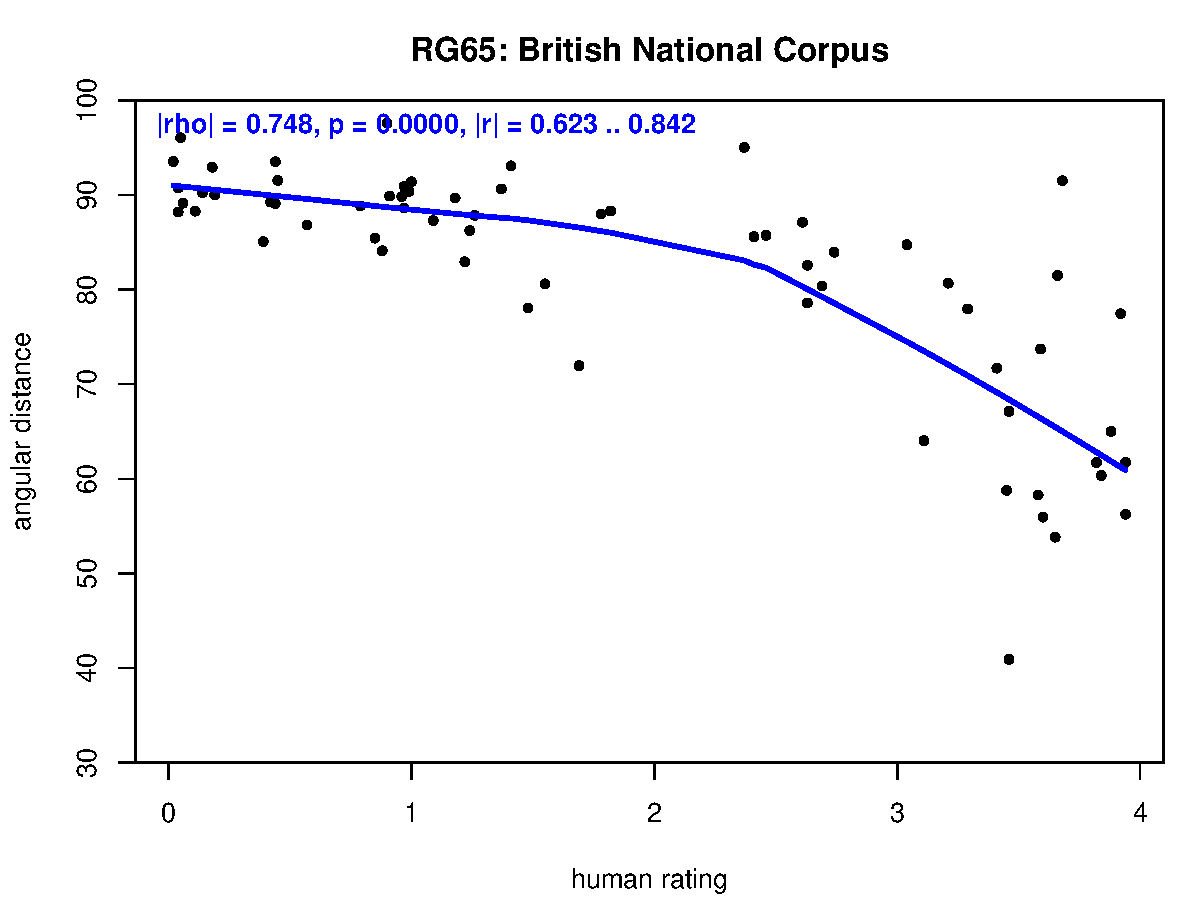
\includegraphics[width=9cm]{img/bnc_rg65}
\end{center}
\end{frame}

\begin{frame}
\frametitle{Semantic similarity judgments: results}
    \begin{center}
      \begin{tabular}{|l|r|}
      \hline
      \emph{model} & $r$\\
      \hline
      \hline
      dep-filtered+SVD & 0.8\\
      \hline
      dep-filtered    & 0.7\\
      \hline
      dep-linked  (DM) & 0.64\\
      \hline
      window & 0.63\\
      \hline
    \end{tabular}

    \gap[1]
    \primary{Results for RG65 task}
      \end{center}
\end{frame}


%%%%%%%%%%%%%%%%%%%%%%%%%%%%%%%%%%%%%%%%%%
%\subsection{Noun categorization}


\begin{frame}
\frametitle{Categorization}

\begin{itemize}
\item In \primary{categorization tasks}, subjects are typically asked to assign experimental items -- objects, images, words -- to a given category or group items belonging to the same category
\begin{itemize}
\item categorization requires an understanding of the relationship between the items in a category
\end {itemize}
\item Categorization is a basic cognitive operation presupposed by further semantic tasks
\begin{itemize}
\item \primary{inference}
\begin{itemize}
\item if X is a CAR then X is a VEHICLE
\end{itemize}
\item \primary{compositionality}
\begin{itemize}
\item $\lambda y:\text{FOOD}\; \lambda x:\text{ANIMATE}; eat(x,y)$
\end{itemize}
\end{itemize}
\item ``Chicken-and-egg'' problem for relationship of categorization and similarity (cf.\ Goodman 1972, Medin et al.\ 1993)
\end{itemize}
\end{frame}


\frame{
\frametitle{Noun categorization}

  \begin{description}
  \item [ Dataset] 44 concrete nouns (ESSLLI 2008 Shared Task)
   \begin{itemize}
  \item 24 natural entities
     \begin{itemize}
    \item 15 animals:\\
      7 birds (\emph{eagle}), 8 ground animals (\emph{lion})
    \item 9 plants: 4 fruits (\emph{banana}), 5 greens (\emph{onion})
    \end{itemize}
  \item 20 artifacts
    \begin{itemize}
    \item 13 tools (\emph{hammer}), 7 vehicles (\emph{car})
    \end{itemize}
  \end{itemize}
\end{description}
\pause

\begin{itemize}
\item DSMs and noun categorization
\begin{itemize}
\item categorization can be operationalized as a \primary{clustering task}
\begin{enumerate}
\item for each noun $w_i$ in the dataset, take its vector $\vw_i$
\item use a \primary{clustering method} to group close vectors $\vw_i$
\item evaluate whether clusters correspond to gold-standard semantic
  classes (purity, entropy, \ldots)
\end{enumerate}

\end{itemize}

\end{itemize}

}




\begin{frame}
\frametitle{Noun categorization}
\begin{itemize}
\item Clustering experiments with CLUTO (Karypis 2003)
\begin{itemize}
\item repeated bisection algorithm
\item 6-way (birds, ground animals, fruits, greens,
tools and vehicles), 3-way (animals, plants and
artifacts) and 2-way (natural and artificial entities) clusterings
\end{itemize}
\pause
\item Clusters evaluation
\begin{itemize}
\item \primary{entropy} -- whether words from different classes are represented in the same cluster (\primary{best = 0})
\item \primary{purity} -- degree to which a cluster contains words from one class only (\primary{best = 1})
\item \primary{global score} across the three clustering experiments
\begin{displaymath}
\sum_{i=1}^3 \text{Purity}_i -  \sum_{i=1}^3 \text{Entropy}_i
\end{displaymath}

\end{itemize}
\end{itemize}
\end{frame}


\begin{frame}
\frametitle{Noun categorization: example}
\ungap[1]
\begin{center}
  \only<beamer:1| handout:0>{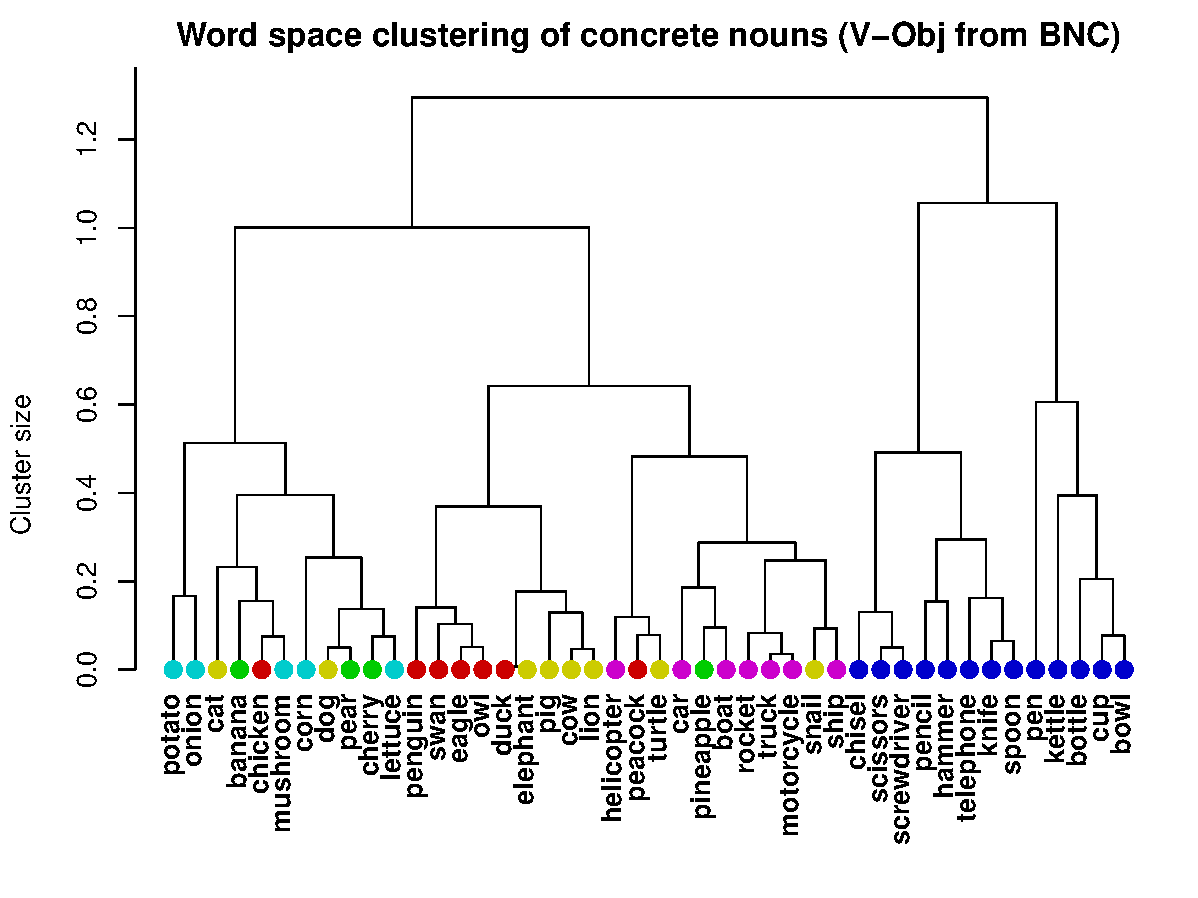
\includegraphics[width=8cm]{img/hieroglyph_clustering}}%
  \only<beamer:2-| handout:1>{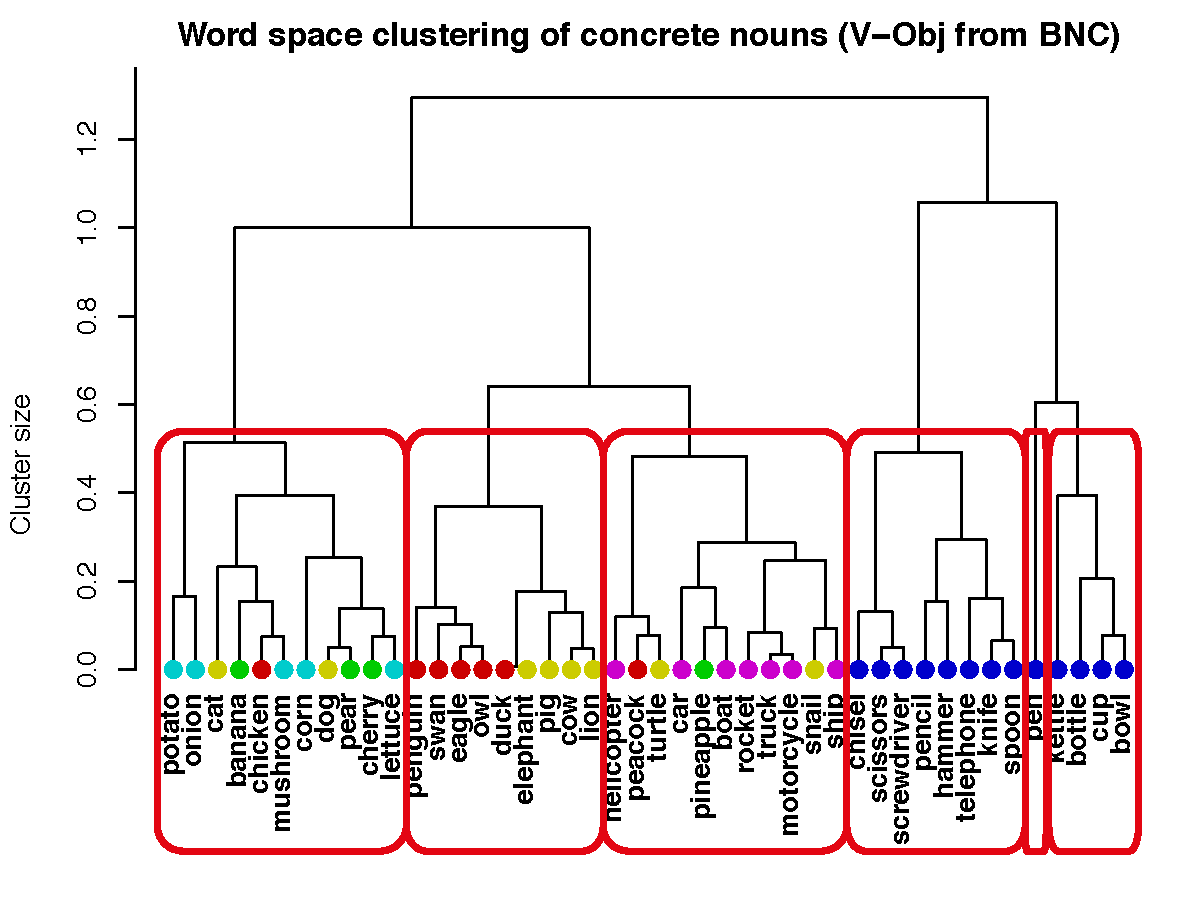
\includegraphics[width=8cm]{img/hieroglyph_clustering_6}}%
\end{center}
\ungap[1]
\begin{itemize}
\item<3-> majority labels: greens, birds, vehicles, tools, tools, tools
\item<3-> correct: 5/11, 5/9, 6/11, 8/8, 1/1, 4/4
\item<4-> purity = 30 correct out of 44 = 68.2\%
\end{itemize}

\end{frame}


\frame{
\frametitle{Noun categorization: results}

 \begin{center}
  \begin{tabular}{|l|r|r||r|r||r|r||r|}
      \hline
      \emph{model} &\multicolumn{2}{|c||}{\emph{6-way}} &  \multicolumn{2}{|c||}{\emph{3-way}} & \multicolumn{2}{|c||}{\emph{2-way}}&  \multicolumn{1}{|c|}{\emph{global}}\\
      \cline{2-7}
      &   \emph{P} & \emph{E}  & \emph{P} & \emph{E}  & \emph{P} & \emph{E} &\\
      \hline
      \hline
      Katrenko & 89 & 13 & 100 & 0 & 80 & 59 & 197\\ 
      \hline
      Peirsman+ & 82 & 23 & 84 & 34 & 86 & 55 & 140\\
      \hline
      dep-typed (DM) & 77 & 24 & 79 & 38 & 59 & 97 & 56\\
      \hline
      dep-filtered & 80 &28 & 75& 51& 61& 95 & 42\\
      \hline
      window & 75& 27&  68& 51& 68& 89   &44\\
      \hline
      Peirsman$-$ & 73 & 28 & 71 & 54 & 61 & 96 & 27\\
      \hline
      Shaoul & 41& 77& 52& 84 & 55& 93& -106\\
      \hline
    \end{tabular}
\end{center}

\begin{center}\footnotesize
  {\tt Katrenko, Peirsman+/-, Shaoul}: ESSLLI 2008 Shared Task\\
  {\tt DM}: Baroni \& Lenci (2009)
\end{center}
     
 
}


%%%%%%%%%%%%%%%%%%%%%%%%%%%%%%%%%%%%%%%%%%\
%\subsection{Semantic priming}

\begin{frame}
  \frametitle{Semantic priming}
  \begin{itemize}
  \item Hearing/reading a ``related'' prime facilitates access to a
    target in various lexical tasks (naming, lexical decision,
    reading)
    \begin{itemize}
  \item  the word \emph{pear} is recognized/accessed faster if it is
    heard/read after \emph{apple}
    \end{itemize}
    \pause
  \item Hodgson (1991) single word lexical decision task, 136
    prime-target pairs (cf.\ Padó \& Lapata 2007)
    \begin{itemize}
  \item similar amounts of priming for different
    semantic relations between primes and targets (approx.~23 pairs
    per relation):
    \begin{itemize}
    \item synonyms (synonym): \emph{to dread/to fear}
    \item antonyms (antonym): \emph{short/tall}
    \item coordinates (coord): \emph{train/truck}
    \item super- and subordinate pairs (supersub): \emph{container/bottle}
    \item free association pairs (freeass): \emph{dove/peace}
    \item phrasal associates (phrasacc): \emph{vacant/building}
    \end{itemize}
  \end{itemize}
\end{itemize}
\end{frame}



\begin{frame}
  \frametitle{Simulating semantic priming}
  \framesubtitle{McDonald \& Brew (2004), Padó \& Lapata (2007)}
 \begin{itemize}
 \item DSMs and semantic priming
  \begin{enumerate}
  \item for each related prime-target pair, 
  measure cosine-based similarity between pair items (e.g.,
    \emph{to dread/to fear})
    \pause
  \item to estimate \primary{unrelated primes}, take average of cosine-based similarity of target with other
    primes from same relation data-set (e.g., \emph{value/to fear})
    \pause
  \item similarity between related items should be significantly higher
    than average similarity between unrelated items
    \item[]
  \end{enumerate}
  \pause
\item Significant effects ($p < .01$) for all semantic relations 
  \begin{itemize}
  \item strongest effects for synonyms, antonyms \& coordinates
  \end{itemize}
  \end{itemize}
\end{frame}


%%%%%%%%%%%%%%%%%%%%%%%%%%%%%%%%%%%%%%%%%%\
\subsection{Relational similarity}


\begin{frame}
  \frametitle{Finding and distinguishing semantic relations}
  \begin{itemize}
  \item Classic distributional semantic models are based on
    \primary{attributional} similarity
    \begin{itemize}
    \item single words/concepts that share attributes / tend to occur
      in the same contexts are semantically similar
    \end{itemize}
  \item Attributional similarity can be modeled with DSMs that have \primary{single words}
  as matrix rows
  \begin{itemize}
  \item matrix columns represent attributes shared by similar words
\end{itemize}
  \end{itemize}
  \pause
   \begin{center}
   \begin{tabular}{l|c|c|c}

         &{\color{counterpoint}die}           &{\color{counterpoint}kill}           &{\color{counterpoint}gun} \\
\hline
{\color{blue}teacher}  &109.4         &0.0             &0.0  \\
{\color{blue}victim}   &1335.2        &22.4            &0.0 \\
{\color{blue}soldier}  &4547.5        &1306.9        &105.9\\
{\color{blue}policeman} &68.6          &38.2           &30.5\\

  \end{tabular}
  \end{center}

  
  
\end{frame}


\begin{frame}
  \frametitle{Attributional and relational similarity}
  \framesubtitle{Turney (2006)}

  \begin{itemize}
  \item \emph{Policeman} is \primary{attributionally} similar to
    \emph{soldier}
    \begin{itemize}
    \item both occur in contexts like:
    \emph{kill X}, \emph{with gun}, \emph{for security}
    \end{itemize}
    \pause
  \item The pair \emph{policeman-gun} is \primary{relationally}
    similar to \emph{teacher-book}
    \begin{itemize}
    \item both are often connected by \emph{with}, \emph{use},
      \emph{of} in context
    \end{itemize}
    \pause
    \item It is not always possible to reduce relational similarity to attributional similarity
    \begin{itemize}
\item \emph{mason}:\emph{stone} :: \emph{carpenter}:\emph{wood}\\
  \vs\ \emph{traffic}:\emph{street} :: \emph{water}:\emph{riverbed}
\begin{itemize}
\item \emph{mason} - \emph{carpenter} and \emph{stone} - \emph{wood} are attributionally similar
\item \emph{traffic} - \emph{water} and \emph{street} - \emph{riverbed} are \primary{not} attributionally similar
\end{itemize}
\end{itemize}

  \end{itemize}
\end{frame}



\begin{frame}
  \frametitle{Finding and distinguishing semantic relations with DSMs}

  \begin{itemize}
    \item Find non-taxonomic semantic relations
      \begin{itemize}
      \item look at direct co-occurrences of \primary{word pairs} in texts (when
        we talk about a concept, we are likely to also mention its
        parts, function, etc.)
      \end{itemize}
      \pause
    \item Distinguish between different semantic relations
      \begin{itemize}
      \item use the contexts of pairs to measure pair similarity, and
        group them into coherent relation types by their contexts
      \item \emph{pairs} that occur in similar contexts (i.e.\
   \primary{connected by similar words and structures}) will tend to be
    related, with the shared contexts acting as a cue to the nature of
    their relation, i.e., measuring their \emph{relational} similarity
    (Turney 2006)
     
      \end{itemize}
  \end{itemize}
\end{frame}


\begin{frame}
  \frametitle{DSMs and relational similarity}
  
 \begin{description}
    \item [rows] \primary{word pairs}
    \item [columns] \primary{syntagmatic links} between the word pairs
    \end{description}

  \begin{center}
        \begin{tabular}{ll|c|c|c|c}
          &        &{\color{counterpoint}in}     &{\color{counterpoint}at}    &{\color{counterpoint}with}&{\color{counterpoint}use}  \\
          \hline
          {\color{secondary}teacher}&{\color{primary}school}  &11894.4&7020.1&28.9 &0.0 \\
          {\color{secondary}teacher}&{\color{primary}handbook}&2.5    &0.0   &3.2  &10.1\\
          {\color{secondary}soldier}&{\color{primary}gun}     &2.8    &10.3  &105.9&41.0\\
        \end{tabular}
      \end{center}
\end{frame}


\begin{frame}
  \frametitle{Recognizing SAT analogies}
    
  \begin{itemize}
\item 374 SAT multiple-choice questions (Turney 2006)
\item Each question  includes 1 target pair (stem) and 5 answer pairs
\item the task is to choose the pair most \emph{analogous} to the stem
  \begin{center}
  \begin{tabular}{ll}
    {\color{secondary}mason} & {\color{secondary}stone}\\
    \hline
    teacher & chalk\\
    \h<2->{carpenter} & \h<2->{wood}\\
    soldier & gun\\
    photograph & camera\\
    book & word\\
  \end{tabular}
  \end{center}
\item<3-> Relational analogue to the TOEFL task
\begin{enumerate}
\item <4-> for each pair $p$, take its row vector $\Vector{p}$
\item <5-> for each stem-pair, select the closest answer-pair\\
  (e.g.\ the one with the highest cosine similarity)
\end{enumerate}
\end{itemize}  
\end{frame}


\begin{frame}
  \frametitle{Recognizing SAT analogies: results}

\begin{center}
 \begin{table}[tbh]
  \begin{small}
    \begin{center}
      \begin{tabular}{|l|r||l|r|}
        \hline
        \emph{model} & \emph{\% correct} & \emph{model} & \emph{\% correct} \\
        \hline
        \hline
        LRA & 56.1&KnowBest & 43.0\\
        \hline
        PERT & 53.3& DM$-$ & 42.3\\
        \hline
        PairClass & 52.1&LSA& 42.0\\
        \hline
        VSM & 47.1&AttrMax & 35.0\\
        \hline
        DM+ & 45.3&AttrAvg & 31.0\\
        \hline
        PairSpace & 44.9&AttrMin & 27.3\\
        \hline
        \emph{k}-means & 44.0&\color{primary}{Random} & \color{primary}{20.0}\\
        \hline
      \end{tabular}
         \end{center}
  \end{small}
\end{table}
  \end{center}


 \begin{center}
  \footnotesize
  {\tt LRA, PERT, PairClass, VSM, KnowBest, LSA}: ACLWiki\\
  {\tt AttrMax, AttrAvg, AttrMin}: Turney(2006)\\
  {\tt DM+, DM-}: Baroni \& Lenci (2009)
\end{center}

\end{frame}

\begin{frame}
  \frametitle{Domain analogies}

  \begin{itemize}
  \item Turney (2008) extends the relational approach to entire
    analogical \emph{domains}
    \begin{center}
      \begin{tabular}{lll}
        solar system&$\rightarrow$& atom \\
        sun&$\rightarrow$& nucleus \\
        planet&$\rightarrow$& electron \\
        mass&$\rightarrow$& charge \\
        attracts&$\rightarrow$& attracts \\
        revolves&$\rightarrow$& revolves \\
        gravity&$\rightarrow$& electromagnetism \\
      \end{tabular}
    \end{center}
\end{itemize}
\end{frame}


\begin{frame}[c]
  \begin{center}
    \textcite{\LARGE Intermission}

    \gap[2]
    Time for a cup of coffee \ldots
  \end{center}
\end{frame}


%%% Local Variables: 
%%% mode: latex
%%% TeX-master: "../workspace"
%%% End: 


\begin{frame}
  \frametitle{Building a distributional model}
  % \framesubtitle{}

  \ungap[2]
  \begin{center}
    pre-processed corpus with linguistic annotation\\
    $\Downarrow$\\
    term-context \vs\ term-term matrix\\
    $\swarrow$ \hspace{3cm} $\searrow$\\
    define targets \& contexts \hspace{2cm} define targets \& features\\
    $\Downarrow$ \hspace{6cm} $\Downarrow$ \\
    \hspace{.5cm} type of context \hspace{1.5cm} type \& size of co-occurrence window\\
    $\searrow$ \hspace{3cm} $\swarrow$\\
    geometric \vs\ probabilistic interpretation\\
    $\Downarrow$\\
    feature scaling\\
    $\Downarrow$\\
    similarity/distance measure + normalisation\\
    $\Downarrow$\\
    dimensionality reduction
  \end{center}
\end{frame}

\begin{frame}
  \frametitle{Building a distributional model}
  % \framesubtitle{}
  
  \footnotesize\centering
  \begin{tikzpicture}
    \node[diagram box=black] (corpus) at (0, 6.5) {pre-processed corpus with linguistic annotation} ;
    \node[diagram box] (tc_terms) at (-3, 5) {define target terms} ;
    \node[diagram box] (tt_terms) at (+3, 5) {define target \& feature terms} ;
    \node[diagram box] (tc_context) at (-3, 4) {context tokens or types} ;
    \node[diagram box] (tt_span) at (+3, 4) {type \& size of co-occurrence} ;
    \node[diagram box=black] (geom_prob) at (0, 3) {$\mathbf{M}$} ;
    \node[diagram box] (scoring) at (-2, 2) {feature scaling} ;
    \node[diagram box] (metric) at (-2, 1) {similarity/distance measure + normalization} ;
    \node[diagram box] (dimred) at (-2, 0) {dimensionality reduction} ;
    \node[diagram ghost] (prob) at (2, 2) {} ;
    \draw[diagram arrow=counterpoint] (corpus) -- node[left=1.5em] {term-context matrix} (tc_terms) ;
    \draw[diagram arrow=counterpoint] (corpus) -- node[right=1.5em] {term-term matrix} (tt_terms) ;
    \draw[diagram arrow] (tc_terms) -- (tc_context) ;
    \draw[diagram arrow] (tt_terms) -- (tt_span) ;
    \draw[diagram arrow] (tc_context) -- (geom_prob) ;
    \draw[diagram arrow] (tt_span) -- (geom_prob) ;
    \draw[diagram arrow=counterpoint] (geom_prob) -- node[left=1.5em] {geometric analysis} (scoring) ;
    \draw[diagram arrow=counterpoint] (geom_prob) -- node[right=1.5em] {probabilistic analysis} (prob) ;
    \draw[diagram arrow] (scoring) -- (metric) ;
    \draw[diagram arrow] (metric) -- (dimred) ;
  \end{tikzpicture}
\end{frame}


\begin{frame}<beamer:10| handout:10>[label=DSM_pipeline]
  \frametitle{Building a distributional model}
  % \framesubtitle{}
  
  \footnotesize\centering
  \begin{tikzpicture}
    \node[diagram box=black] (corpus) at (0, 6.5) {pre-processed corpus with linguistic annotation} ;
    \visible<beamer:2-| handout:2->{
      \node[diagram box] (tt_terms) at (+3, 5) {define target \& feature terms} ;
      \draw[diagram arrow=counterpoint] (corpus) -- node[right=1.5em] {term-term matrix} (tt_terms) ;
    }
    \visible<beamer:3-| handout:3->{
      \node[diagram box] (tt_span) at (+3, 4) {type \& size of co-occurrence} ;
      \draw[diagram arrow] (tt_terms) -- (tt_span) ;
    }
    \visible<beamer:4-| handout:4->{
      \node[diagram box=black] (geom_prob) at (0, 3) {$\mathbf{M}$} ;
      \draw[diagram arrow] (tt_span) -- (geom_prob) ;
    }
    \visible<beamer:5-| handout:5->{
      \node[diagram box] (tc_terms) at (-3, 5) {define target terms} ; 
      \draw[diagram arrow=counterpoint] (corpus) -- node[left=1.5em] {term-context matrix} (tc_terms) ;
    }
    \visible<beamer:6-| handout:6->{
      \node[diagram box] (tc_context) at (-3, 4) {context tokens or types} ;
      \draw[diagram arrow] (tc_terms) -- (tc_context) ;
      \draw[diagram arrow] (tc_context) -- (geom_prob) ;
    }
    \visible<beamer:7-| handout:7->{
      \node[diagram ghost] (prob) at (2, 2) {} ;
      \draw[diagram arrow=counterpoint] (geom_prob) -- node[right=1.5em] {probabilistic analysis} (prob) ;
    }
    \visible<beamer:8-| handout:8->{
      \node[diagram box] (scoring) at (-2, 2) {feature scaling} ;
      \draw[diagram arrow=counterpoint] (geom_prob) -- node[left=1.5em] {geometric analysis} (scoring) ;
    }
    \visible<beamer:9-| handout:9->{
      \node[diagram box] (metric) at (-2, 1) {similarity/distance measure + normalization} ;
      \draw[diagram arrow] (scoring) -- (metric) ;
    }
    \visible<beamer:10-| handout:10->{
      \node[diagram box] (dimred) at (-2, 0) {dimensionality reduction} ;
      \draw[diagram arrow] (metric) -- (dimred) ;
    }
  \end{tikzpicture}
\end{frame}
\againframe<beamer:3| handout:3>{DSM_pipeline}



%%%%%%%%%%%%%%%%%%%%%%%%%%%%%%%%%%%%%%%%%%%%%%%%%%%%%%%%%%%%%%%%%%%%%%
%% References (if any)

\frame[allowframebreaks]{
  \frametitle{References}
  \bibliographystyle{natbib-stefan}
  \begin{scriptsize}
    \bibliography{dsm,stefan-literature,stefan-publications}
  \end{scriptsize}
}

\end{document}

